% Executive Summary of the MSc thesis submitted to Politecnico di Milano
\documentclass[11pt,a4paper,twocolumn]{article}

\usepackage{titlesec}
\usepackage{color}
\usepackage[utf8]{inputenc}
\usepackage[english]{babel}
\usepackage[T1]{fontenc}
\usepackage{graphicx}
\graphicspath{{Images/}}
\usepackage{eso-pic}
\usepackage{subfig}
\usepackage{caption}
\usepackage{iftex}
\ifPDFTeX
\usepackage{transparent}
\else
\newcommand{\transparent}[1]{}
\fi
\usepackage{amsmath}
\usepackage{amsthm}
\usepackage{bm}
\usepackage[overload]{empheq}
\usepackage{tabularx}
\usepackage{booktabs}
\usepackage{longtable}
\usepackage{colortbl}
\usepackage[colorlinks=true,linkcolor=black,anchorcolor=black,citecolor=black,filecolor=black,menucolor=black,runcolor=black,urlcolor=black]{hyperref}
\usepackage{cleveref}
\usepackage[square,numbers,sort&compress]{natbib}
\bibliographystyle{plain}
\usepackage{appendix}
\usepackage{enumitem}
\usepackage{amsthm,thmtools,xcolor}
\usepackage{comment}
\usepackage{fancyhdr}
\usepackage{tcolorbox}
\usepackage{stfloats}
\usepackage{float}

\input{Configuration_files/config}

\renewcommand{\title}{Behavioral Evaluation of Discrete Image Tokenizers}
\renewcommand{\author}{Farzin Nasiri Safarzadeh}
\newcommand{\course}{Mathematical Engineering - Ingegneria Matematica}
\newcommand{\advisor}{Prof. Matteo Matteucci}
\newcommand{\firstcoadvisor}{Paolo Cudrano}
\newcommand{\YEAR}{2025--2026}

\newcommand{\llamagen}{LlamaGen}
\newcommand{\vqgan}{VQGAN}
\newcommand{\imagenet}{ImageNet}

\begin{document}

\input{Configuration_files/title_page}

\section{Motivation and Scope}
\label{sec:motivation}

Autoregressive image generation relies on a discrete tokenizer to convert an image into a sequence of codebook indices. The transformer sees only this sequence: any information discarded, destabilized, or spatially redistributed by the tokenizer becomes a constraint on the generative model that follows. Tokenizers are nevertheless selected primarily through reconstruction quality. That baseline is necessary, but it does not reveal whether nearby images receive stable codes, whether a local intervention remains local, or whether the codebook is used consistently outside the training distribution.

This thesis evaluates discrete image tokenizers as behavioral components rather than only as compression modules. The comparison concerns two public tokenizers used in autoregressive visual generation: the tokenizer released with \vqgan{} \cite{esser2021taming} and the tokenizer released with \llamagen{} \cite{sun2024llamagen}. Both map a $256\times256$ image to a $16\times16$ token grid with a nominal codebook of 16,384 entries. Holding these interface dimensions fixed makes it possible to compare reconstruction, stability, spatial response, and off-distribution usage without conflating them with sequence length or vocabulary size.

The study is organized around five research questions:
\begin{enumerate}[leftmargin=*,label=\textbf{RQ\arabic*:},itemsep=2pt,topsep=3pt]
    \item How much information does each tokenizer preserve, and how fully does it use its codebook?
    \item How stable are token assignments under global image perturbations?
    \item Does a local image-space perturbation produce a local encoder response?
    \item Does a local token-space edit produce a local decoder response?
    \item How do reconstruction quality and code usage change under dataset shift?
\end{enumerate}

The central distinction is between fidelity and behavior. Fidelity asks whether the decoded image resembles the input. Behavioral probes ask how the discrete representation changes when the input, the token grid, or the data distribution changes. The result is not a single ranking criterion. It is a profile of properties that matter for a tokenizer placed before an autoregressive model.

\section{Experimental Design}
\label{sec:design}

\subsection{Tokenizers and reference data}

The \vqgan{} tokenizer uses a 256-dimensional codebook and a perceptual--adversarial training objective. The \llamagen{} tokenizer uses eight-dimensional, $\ell_2$-normalized code vectors and was designed for next-token image generation. The experiments use the released checkpoints rather than retraining either model. This preserves the behavior of the systems as they are distributed, but it also means that architectural and training differences cannot be isolated causally.

The in-distribution reference is the 50,000-image \imagenet{} validation set \cite{deng2009imagenet}. Distribution-shift experiments add ImageNet-V2 \cite{recht2019imagenet}, ImageNet-Sketch \cite{wang2019learning}, ObjectNet \cite{barbu2019objectnet}, BloodMNIST and OrganAMNIST from MedMNIST v2 \cite{yang2023medmnist}, and RVL-CDIP document images \cite{harley2015rvlcdip}. These sets span resampling shift, drawing style, viewpoint and background bias, biomedical imagery, and scanned documents.

\begin{table}[H]
\centering
\caption{Common tokenizer interface and evaluation data.}
\label{tab:setup}
\small
\setlength{\tabcolsep}{2.5pt}
\begin{tabular}{@{}lrr@{}}
\toprule
\textbf{Item} & \textbf{\llamagen{}} & \textbf{\vqgan{}} \\
\midrule
Input resolution & $256\times256$ & $256\times256$ \\
Token grid & $16\times16$ & $16\times16$ \\
Codebook size & 16,384 & 16,384 \\
Code dimension & 8 & 256 \\
\midrule
\multicolumn{3}{@{}l}{\textbf{Dataset sizes}} \\
ImageNet / ImageNet-V2 & \multicolumn{2}{r}{50,000 / 10,000} \\
Sketch / ObjectNet & \multicolumn{2}{r}{50,889 / 50,273} \\
Blood / Organ / RVL & \multicolumn{2}{r}{17,092 / 57,187 / 39,996} \\
\bottomrule
\end{tabular}
\end{table}

\subsection{Measurements and interventions}

Reconstruction is measured with PSNR, SSIM, LPIPS, and FID. PSNR and SSIM emphasize pixel and structural agreement; LPIPS measures perceptual distance; FID compares the distributions of reference and reconstructed images. FID is interpreted only within the same dataset because its scale depends on the reference distribution. The baseline figure retains four supporting set-level diagnostics from the evaluator: spatial FID (sFID), feature-space precision and recall, and Inception Score. They respectively describe spatial distribution match, fidelity and coverage of the reference feature manifold, and classifier confidence combined with predicted-class diversity; they are treated as secondary diagnostics rather than substitutes for paired reconstruction metrics.

Code usage is computed from all assignments in a dataset. An entry is active if it appears at least once. To separate isolated assignments from sustained use, an effective-active threshold of $10^{-6}$ of all assignments is also reported; on \imagenet{}, this corresponds to at least 13 occurrences among 12.8 million tokens. Usage concentration is summarized by perplexity and by the mass assigned to the 10, 100, and 500 most frequent codes.

Three controlled interventions complement the baseline. First, isotropic Gaussian noise is added to the whole image and token flips are measured against the clean encoding. Second, noise is restricted to an $8\times8$ region of the $16\times16$ token grid and token changes are split into inside- and outside-patch regions. The far field contains token cells at Manhattan distance at least six from the patch. Third, selected tokens are replaced using embedding-space relations. Decoder response is the channel-averaged root-mean-square pixel change relative to the clean reconstruction; its inside and outside means, $\Delta_{\mathrm{in}}$ and $\Delta_{\mathrm{out}}$, define the decoder leakage ratio $\lambda_{\mathrm{dec}}=\Delta_{\mathrm{out}}/(\Delta_{\mathrm{in}}+\varepsilon)$. For distribution shift, all datasets pass through the same frozen tokenizer and preprocessing pipeline; the resulting frequency distributions are compared with Jensen--Shannon divergence (JSD), active-set retention, perplexity ratios, and top-$k$ concentration.

\section{Reconstruction and Code Use (RQ1)}
\label{sec:rq1}

On \imagenet{}, \llamagen{} reconstructs more faithfully than \vqgan{} on every reported metric: PSNR is 20.79 rather than 19.65, SSIM is 0.558 rather than 0.489, LPIPS is 0.228 rather than 0.286, and FID is 2.19 rather than 5.06. The margins are not interchangeable---each metric emphasizes a different aspect of fidelity---but their agreement establishes a consistent baseline advantage for \llamagen{}.

The two tokenizers reach this result with very different codebook usage. \llamagen{} activates all 16,384 entries on \imagenet{}, with 16,384 effectively active entries and perplexity 16,179. \vqgan{} activates 972 entries, of which 971 pass the effective threshold, with perplexity 910. Thus, about 94\% of the nominal \vqgan{} vocabulary is inactive for this checkpoint and dataset. Its top 500 entries account for 66.5\% of all assignments, compared with 4.6\% for \llamagen{}. The difference is therefore not merely whether an index appears: \vqgan{} concentrates repeated use in a much smaller vocabulary, while \llamagen{} distributes assignments across almost the entire codebook.

Equal nominal codebook size therefore does not imply equal empirical capacity. The released checkpoints expose the same index range, but their active vocabularies differ by more than an order of magnitude. Reconstruction fidelity and codebook use must be reported together.

\begin{figure*}[t]
    \centering
    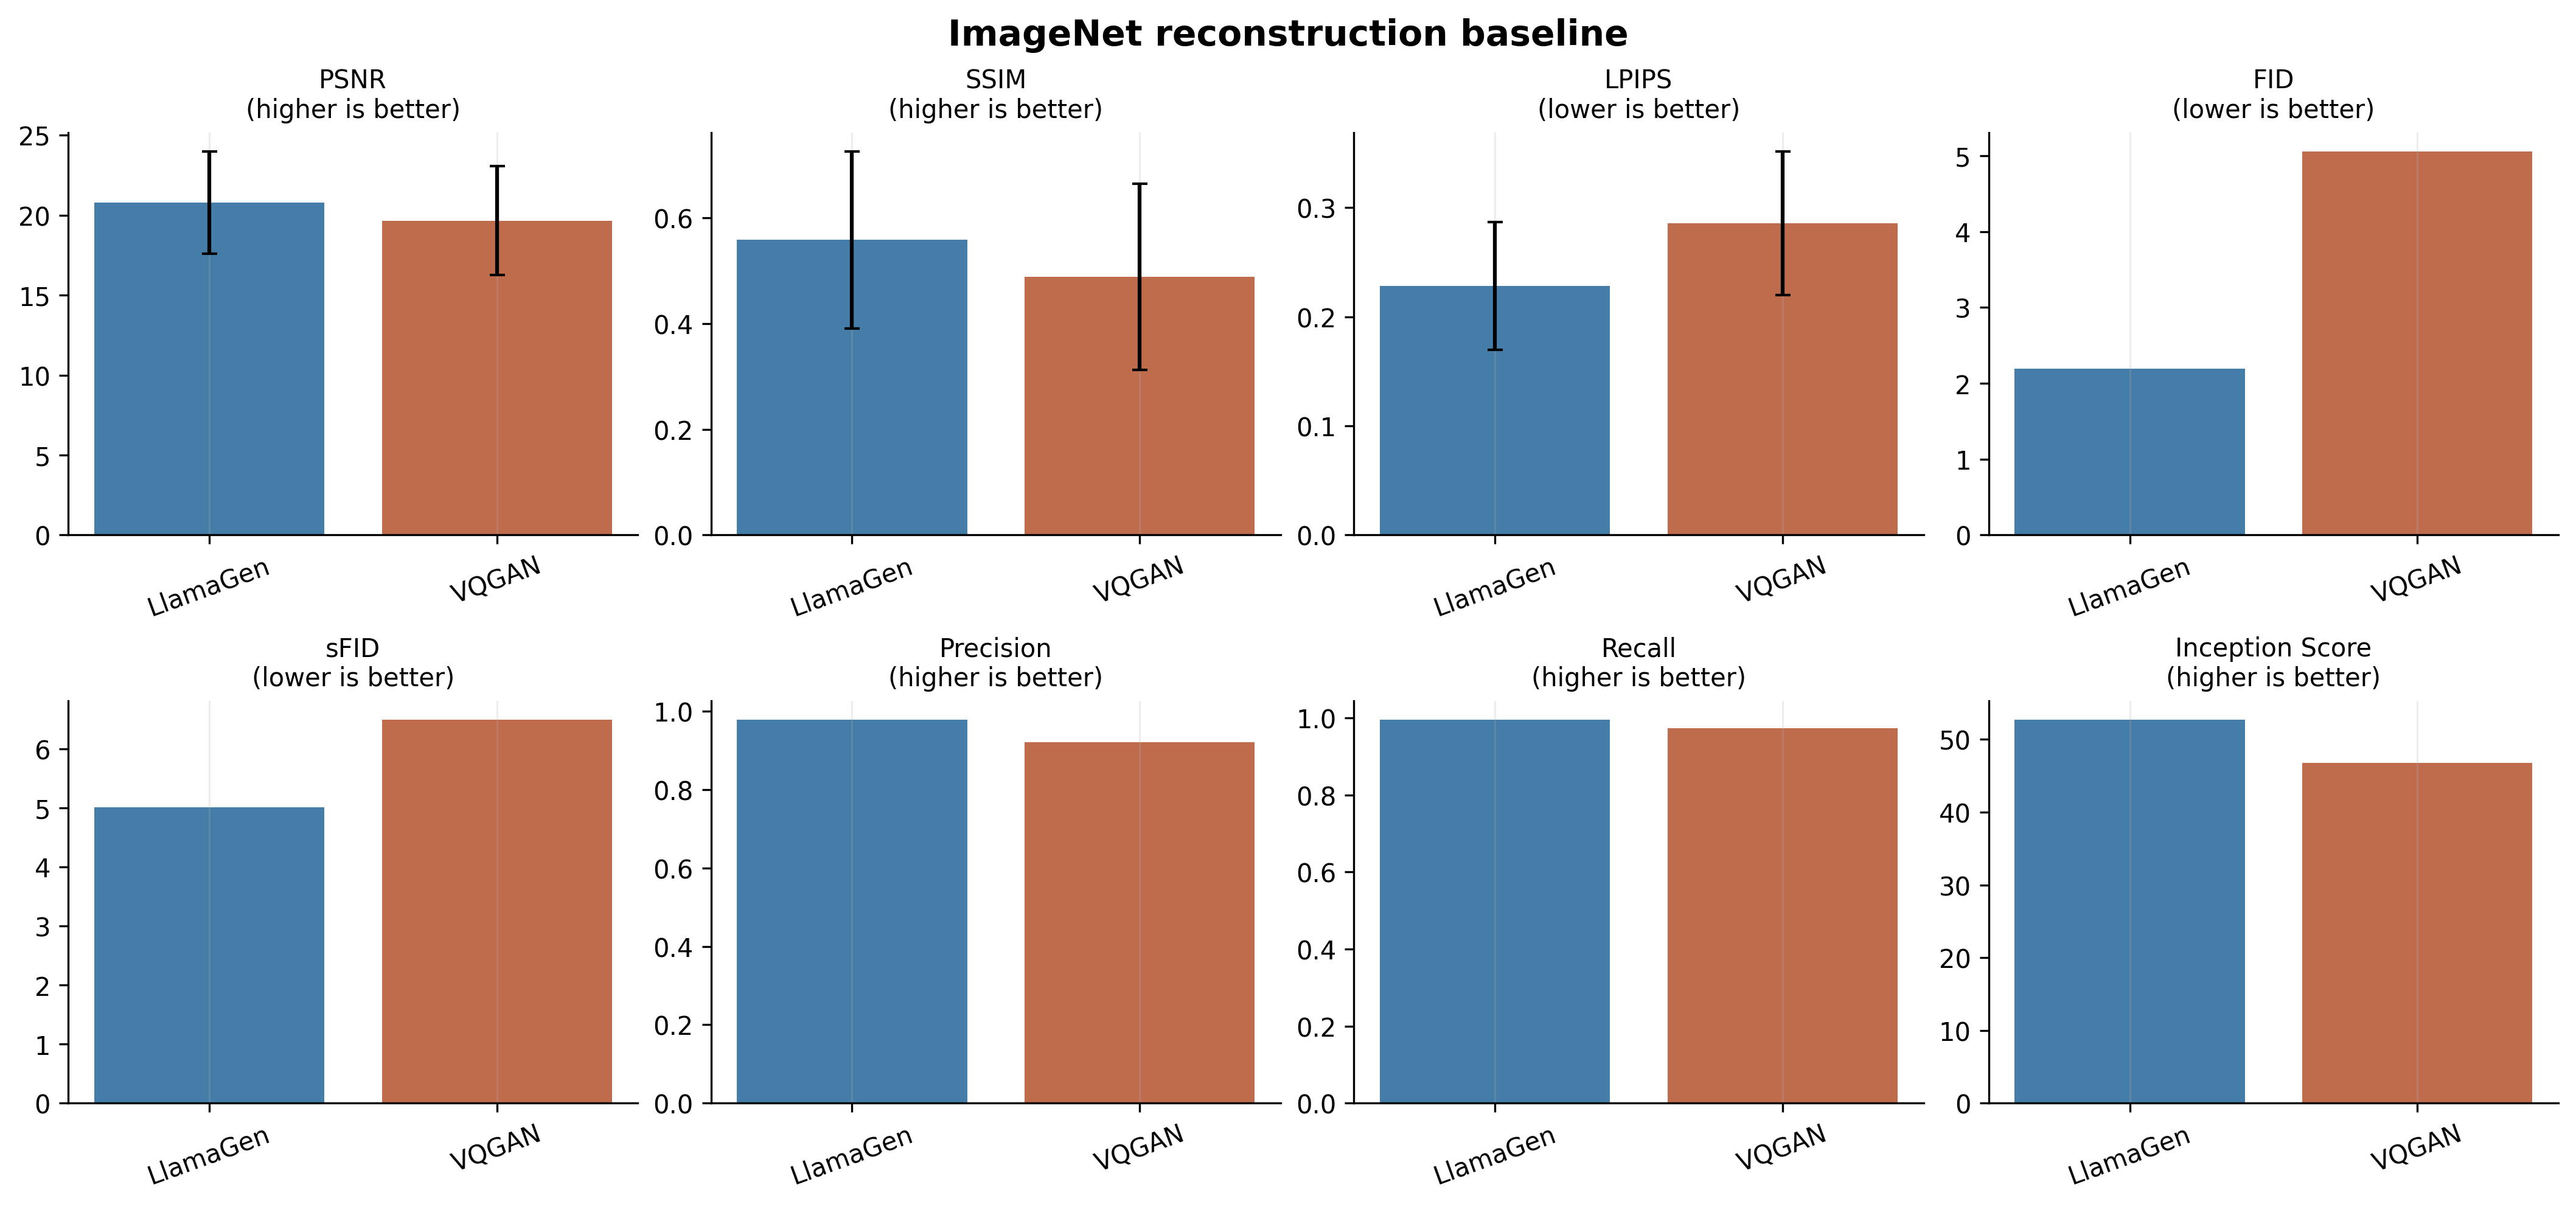
\includegraphics[width=0.94\textwidth]{rq1_reconstruction_metrics.png}
    \caption{Reconstruction metrics on the \imagenet{} validation set. Error bars show the standard deviation of per-image metrics; FID is a dataset-level quantity.}
    \label{fig:rq1}
\end{figure*}

\section{Global Robustness (RQ2)}
\label{sec:rq2}

Global Gaussian noise reveals that high reconstruction quality does not imply stable discrete assignments. With images represented in $[0,1]$, a standard deviation of $\sigma=0.1$ flips 79.5\% of \llamagen{} tokens and 75.1\% of \vqgan{} tokens. At $\sigma=0.2$, the rates rise to 91.0\% and 89.0\%; at $\sigma=0.5$, both exceed 97\%. Because the two quantizers use different latent geometries, these raw rates describe checkpoint behavior rather than a calibrated cross-model robustness scale. They nevertheless show that both representations cross code boundaries frequently under visually modest global changes.

The reconstructed images degrade more gradually than the token grids. At $\sigma=0.5$, PSNR against the clean reconstruction remains 16.22 for \llamagen{} and 14.90 for \vqgan{}. Many index changes therefore map to decoder outputs that remain perceptually related. Token equality is a stricter notion than image-level stability.

Noise also compresses the usage distribution. \llamagen{} perplexity falls from 16,179 to 6,434 between the clean condition and $\sigma=0.5$, while \vqgan{} falls from 910 to 560. Over the same range, top-100 mass rises from 0.012 to 0.115 for \llamagen{} and from 0.165 to 0.388 for \vqgan{}. Global corruption does not simply randomize the representation; it makes both tokenizers rely more heavily on a smaller subset of codes.

\begin{figure*}[t]
    \centering
    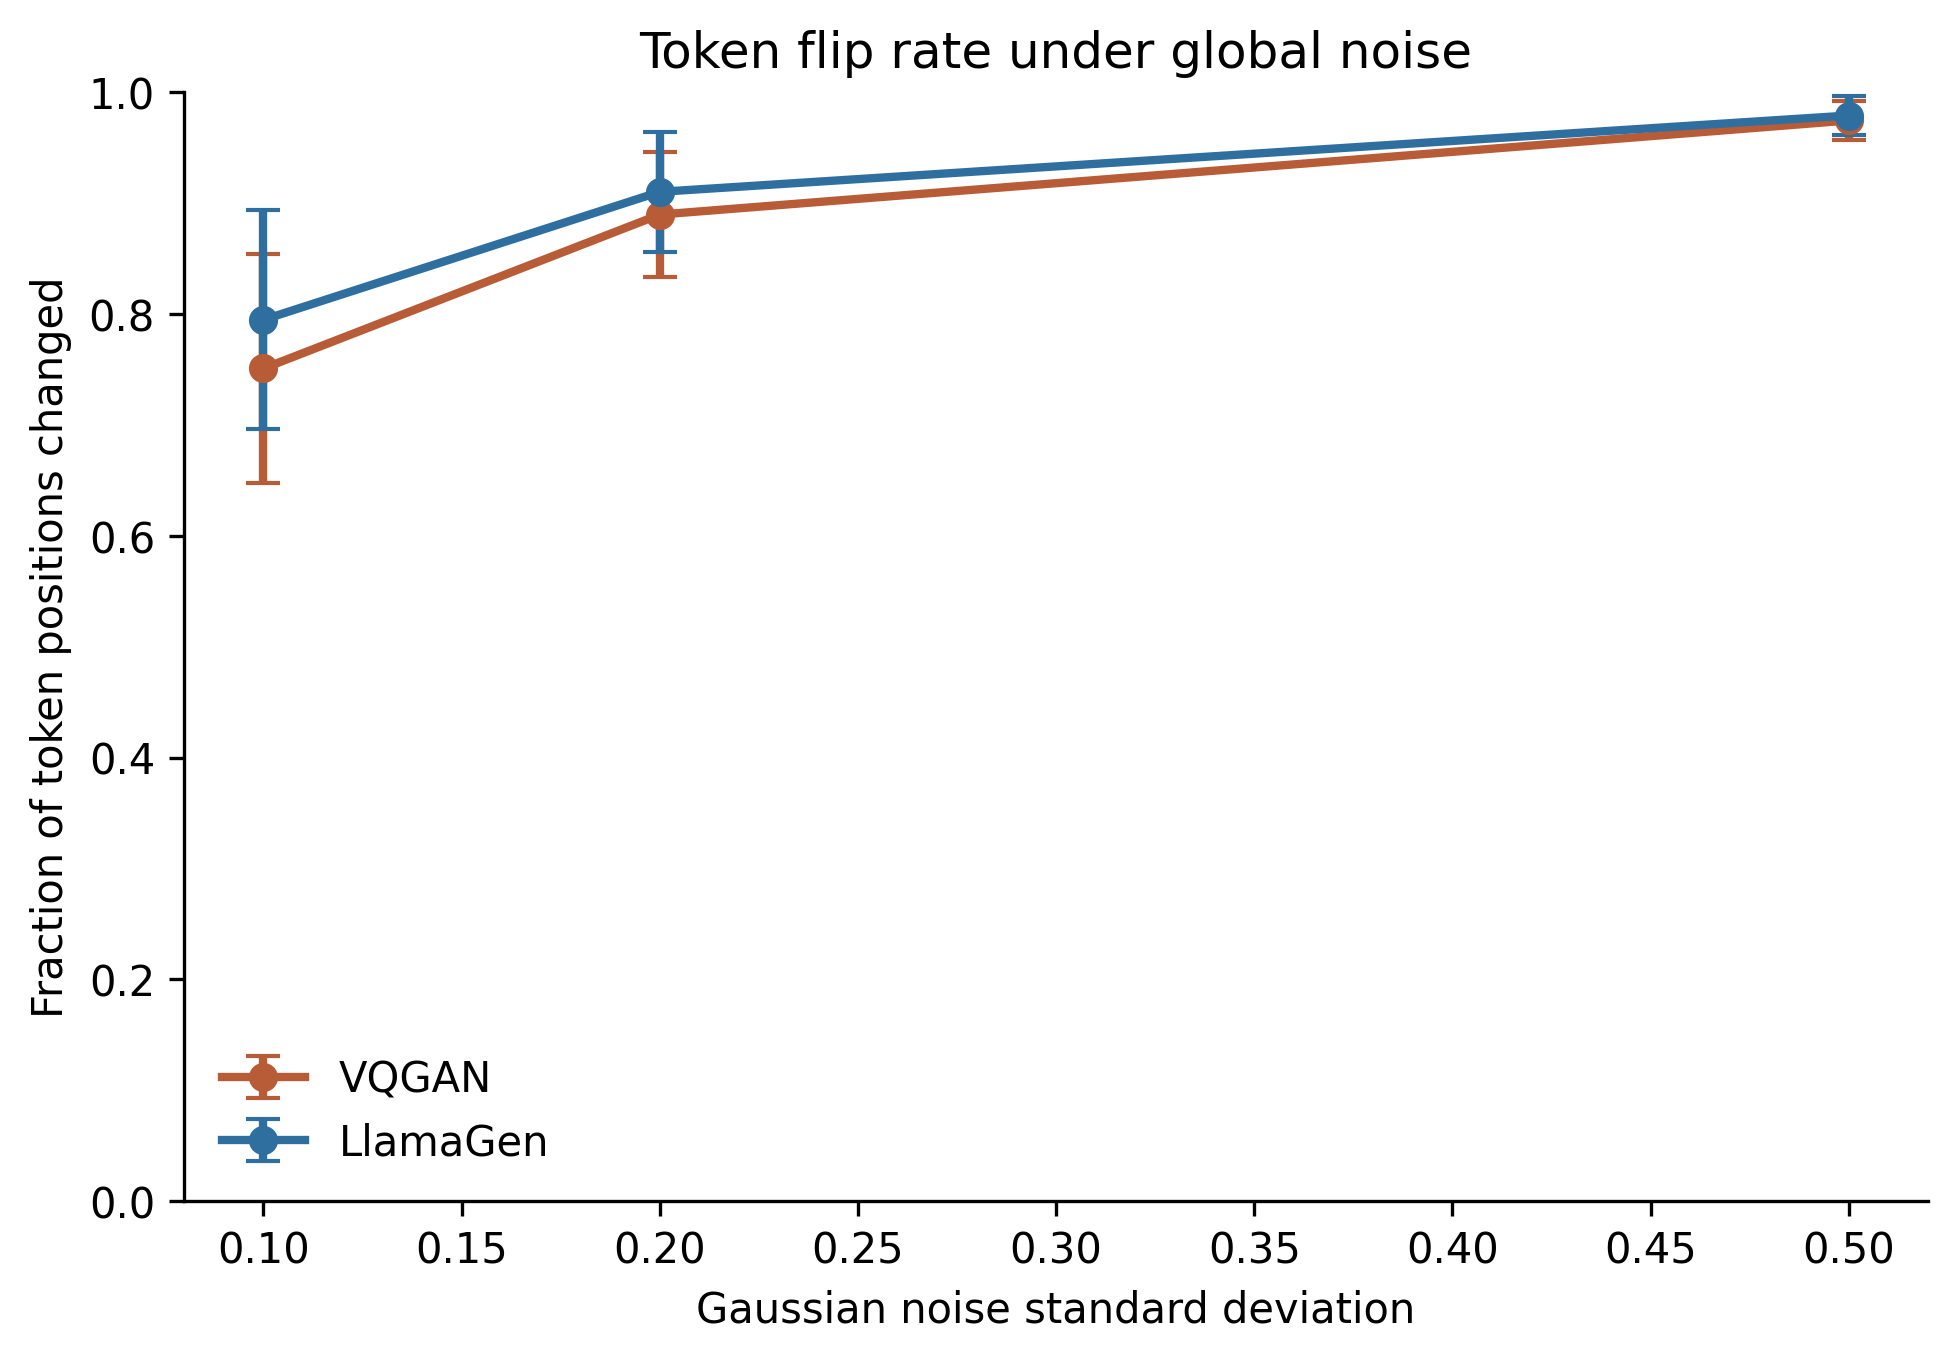
\includegraphics[width=0.92\textwidth]{rq2_token_flip_vs_sigma.png}
    \caption{Mean token-flip rate under global Gaussian noise. Error bars summarize variation across images.}
    \label{fig:rq2}
\end{figure*}

Discrete token identity is therefore much less stable than decoded appearance. The perturbations also induce systematic concentration rather than uniform code replacement. A tokenizer used for autoregressive modeling should be assessed both at the index level and after decoding.

\section{Encoder Locality (RQ3)}
\label{sec:rq3}

The encoder-locality probe applies noise only inside an image patch and measures where token assignments change. The main $8\times8$ token-space patch covers one quarter of the grid. A perfectly local encoder would alter only token cells whose receptive fields overlap that patch. Neither checkpoint behaves this way. At the lowest noise level, $\sigma=0.1$, the mean far-field flip rate is 17.4\% for \vqgan{} and 17.8\% for \llamagen{}. At $\sigma=0.25$, outside-patch flip rates reach 44.1\% and 42.8\%; at $\sigma=0.5$, they reach 52.1\% and 50.5\%. Replacing the patch with a constant masked region produces outside rates of 56.3\% and 49.5\%.

\begin{figure*}[t]
    \centering
    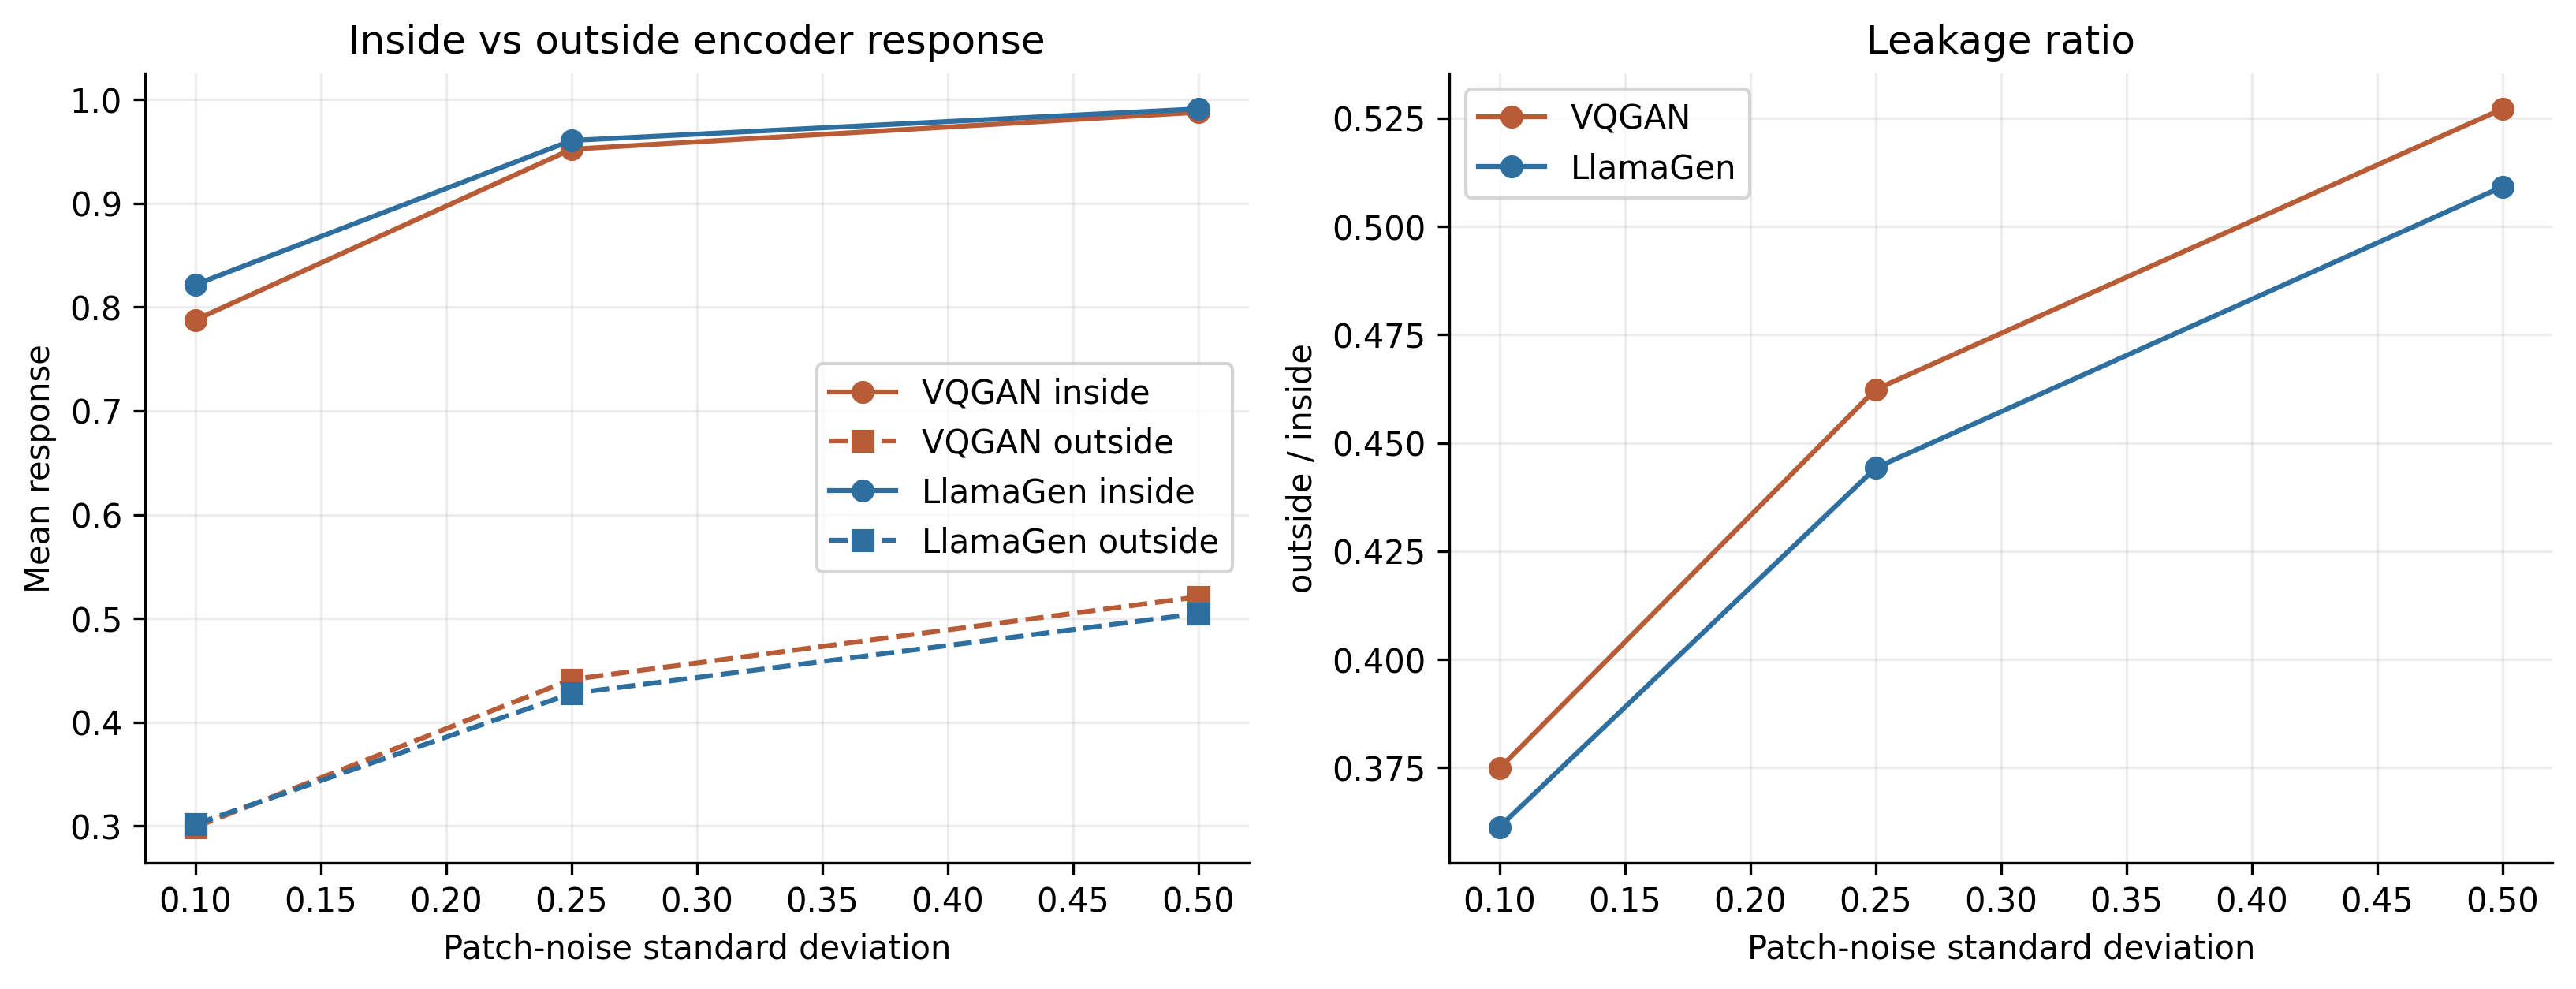
\includegraphics[width=0.94\textwidth]{rq3_encoder_locality.png}
    \caption{Inside- and outside-patch token responses to local image-space interventions. A substantial outside response remains for both tokenizers.}
    \label{fig:rq3}
\end{figure*}

The result is not explained by a one-cell boundary effect. The response extends beyond the perturbed region and remains visible in far-field summaries. Convolutional receptive fields, downsampling, normalization, and nearest-neighbor quantization can all contribute, but the experiment does not isolate their individual roles. What it establishes is the behavior of the released encoder--quantizer pipelines: a local change in the image is represented by a partly global change in token identity.

A $16\times16$ index map preserves coarse layout, but an individual token cannot be assumed to depend only on its corresponding image patch. Local token attribution and localized conditioning methods should account for this encoder-side leakage.

\section{Decoder Locality (RQ4)}
\label{sec:rq4}

The reverse intervention edits the token grid directly and measures where the decoded image changes. Replacement codes are selected from precomputed embedding-space relations: close alternatives test small moves in the codebook, while orthogonal, random, and farthest alternatives test increasingly disruptive substitutions. Edits cover controlled fractions of the grid, and image response is separated into the edited and unedited regions.

At a 25\% edit fraction with the closest replacement mode, \llamagen{} obtains PSNR 20.36 and LPIPS 0.134, compared with 20.00 and 0.182 for \vqgan{}. For the farthest 75\% intervention, the gap becomes much larger: \llamagen{} reaches PSNR 7.74 and LPIPS 0.702, whereas \vqgan{} reaches PSNR 3.74 and LPIPS 0.790. The ordering agrees with the reconstruction baseline: \llamagen{} tolerates token substitutions better, especially when replacements are distant and numerous.

\begin{figure*}[t]
    \centering
    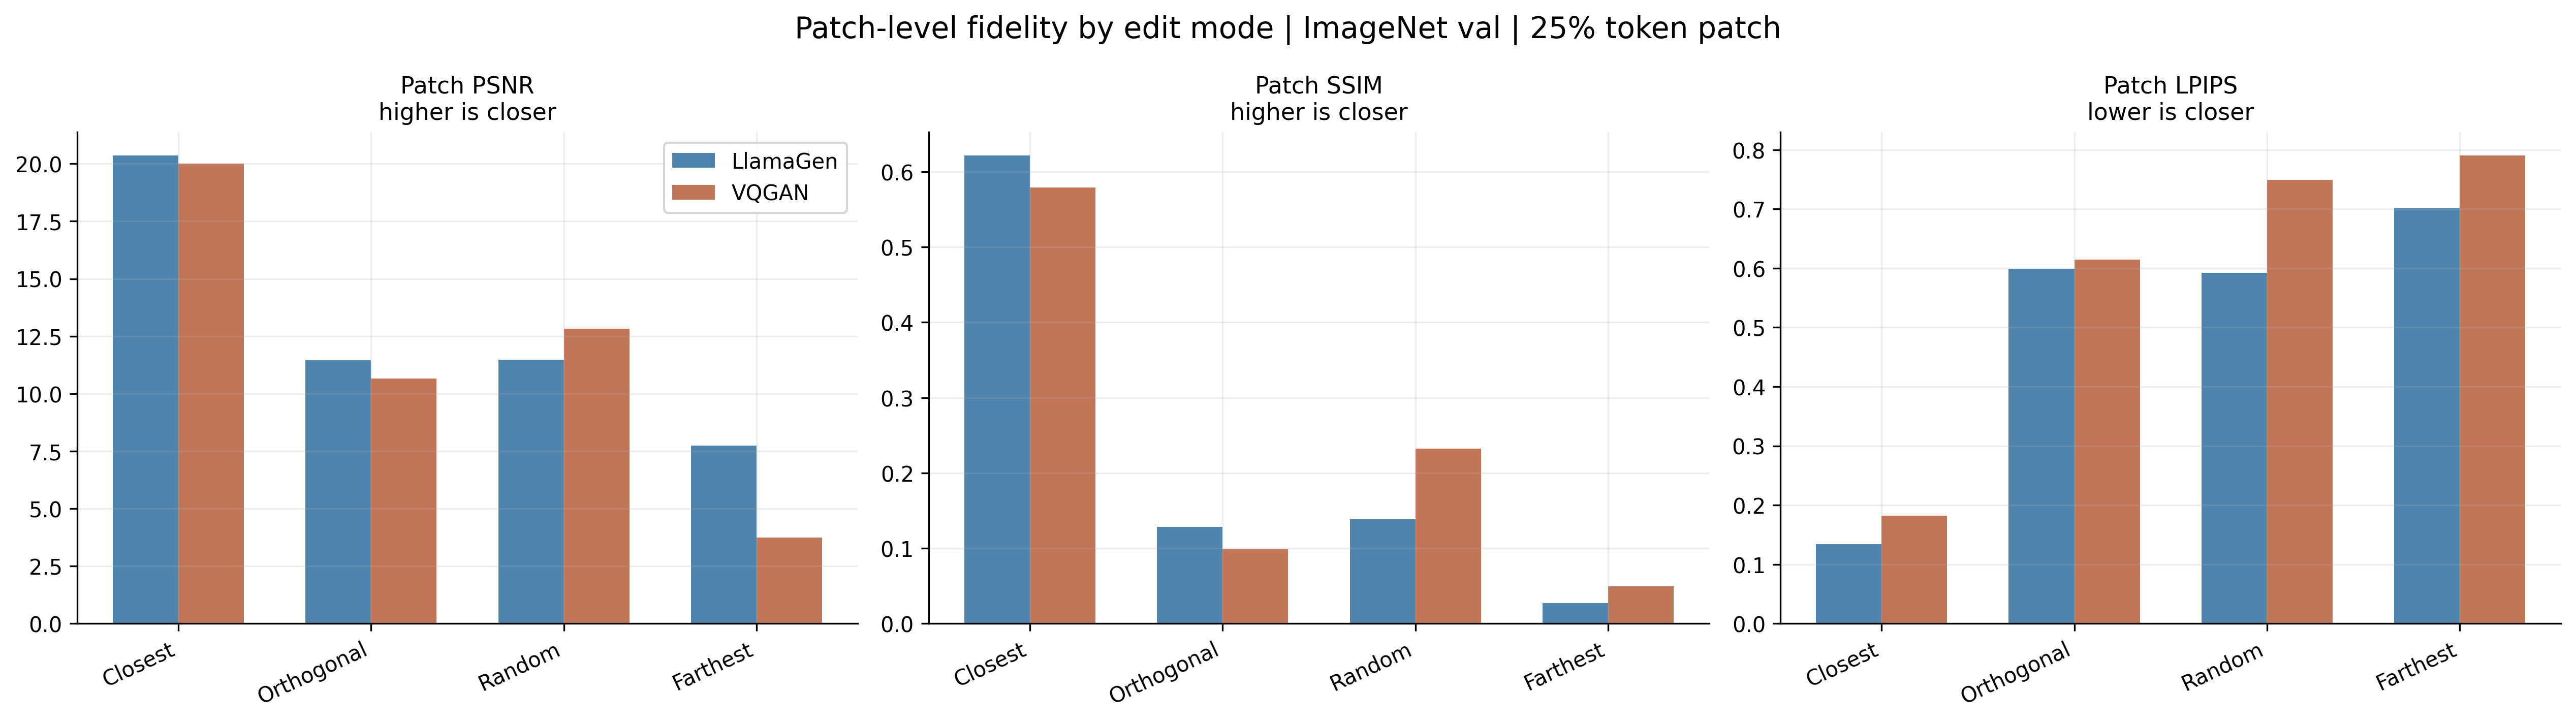
\includegraphics[width=0.94\textwidth]{rq4_decoder_fidelity.png}
    \caption{Decoder-only edit fidelity at a 25\% edit fraction. Replacement geometry strongly affects the decoded response.}
    \label{fig:rq4}
\end{figure*}

Decoder response is not confined to the edited cells. At a 25\% edit fraction, the median decoder leakage ratio $\lambda_{\mathrm{dec}}$ is 0.141 for \llamagen{} and 0.148 for \vqgan{} in the farthest mode; for \vqgan{}, even the closest mode reaches 0.263. The exact magnitude depends on the edit mask and replacement relation, but the qualitative result is stable: local token edits can have non-local image consequences.

Repeating the protocol on ImageNet-V2 produces nearly identical aggregate trends. Across modes, the largest LPIPS change is 0.0068, the largest absolute outside-response change is 0.0016, and PSNR remains within 0.17 dB. The decoder-side finding is therefore not an artifact of one \imagenet{} sample set. The encoder and decoder probes together reveal an asymmetric but consistent picture: spatial indexing is useful, yet neither direction of the tokenizer is strictly local.

\section{Distribution Shift (RQ5)}
\label{sec:rq5}

The final study asks whether a tokenizer uses the same discrete vocabulary when the image distribution changes. Active-set overlap alone suggests strong stability. \llamagen{} retains all \imagenet{}-active codes on ImageNet-V2, ImageNet-Sketch, ObjectNet, and OrganAMNIST, 98.4\% on BloodMNIST, and 99.4\% on RVL-CDIP. For \vqgan{}, the same 972 entries remain active on ImageNet-V2, ImageNet-Sketch, ObjectNet, and OrganAMNIST; retention is 99.4\% on BloodMNIST and 99.9\% on RVL-CDIP.

This near-perfect overlap is not evidence that the distributions are unchanged. Frequency-sensitive measures reveal a graded shift. For \llamagen{}, JSD from \imagenet{} is 0.0020 on ImageNet-V2, 0.0200 on ObjectNet, 0.1035 on OrganAMNIST, 0.1531 on ImageNet-Sketch, 0.2260 on BloodMNIST, and 0.2510 on RVL-CDIP. Its perplexity ratio relative to \imagenet{} falls from 0.995 on ImageNet-V2 to 0.230 on RVL-CDIP. \vqgan{} shows the same ordering at a lower effective vocabulary size: JSD ranges from 0.0004 on ImageNet-V2 to 0.1949 on RVL-CDIP, while the perplexity ratio falls from 1.001 to 0.325.

\begin{figure*}[t]
    \centering
    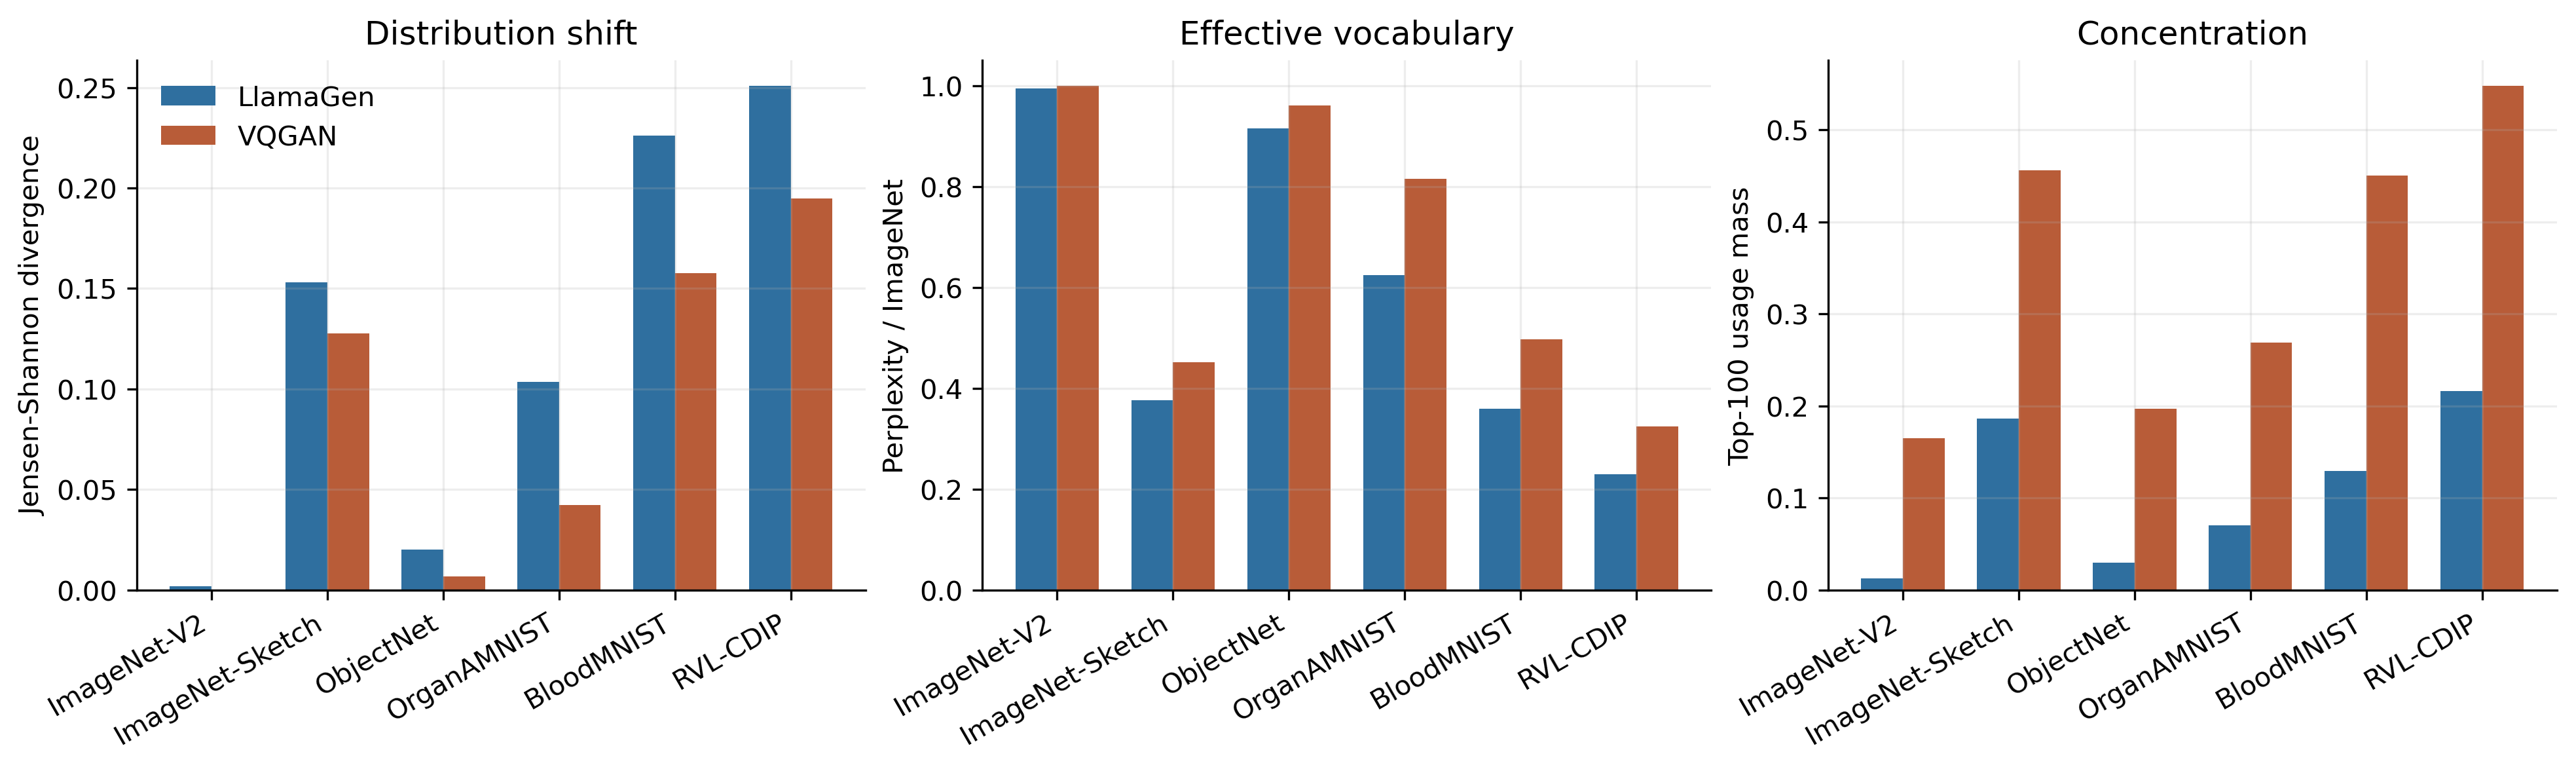
\includegraphics[width=0.96\textwidth]{rq5_distribution_shift.png}
    \caption{Global code-usage shift relative to \imagenet{}. Active vocabularies are largely retained, while frequency divergence and concentration increase with domain distance.}
    \label{fig:rq5}
\end{figure*}

Top-100 mass makes the concentration change concrete. From \imagenet{} to RVL-CDIP, it rises from 0.012 to 0.216 for \llamagen{} and from 0.165 to 0.548 for \vqgan{}. The off-distribution datasets do not generally activate a new vocabulary; they redistribute probability toward a smaller set of familiar codes.

Reconstruction metrics must be read separately from these usage statistics. ImageNet-V2 and ObjectNet remain close to the reference baseline, whereas the medical and document datasets exhibit different pixel statistics and semantics. On OrganAMNIST, for example, both models obtain high PSNR and SSIM but poor FID: FID is 57.16 for \llamagen{} and 76.12 for \vqgan{}. High sample-wise fidelity can coexist with a poor match between reconstructed and reference feature distributions. Across every evaluated dataset, however, \llamagen{} retains the better FID and generally the better reconstruction metrics.

The distribution-shift study therefore changes the interpretation of ``active code.'' A binary alive/dead count is useful for detecting collapse, as in the \vqgan{} baseline, but it is too coarse for shift analysis. Frequency divergence and concentration expose changes that active-set overlap does not.

\section{Limitations}
\label{sec:limitations}

The experiments compare one released checkpoint per tokenizer. Differences therefore combine architecture, latent dimension, normalization, losses, training data, and optimization; the thesis measures deployed behavior but does not identify a single causal mechanism. Raw token-flip rates are also not a calibrated distance across quantizers, because their codebook geometries differ.

All datasets pass through a common $256\times256$ preprocessing pipeline. This supports controlled comparison, but resizing and cropping can distort medical, document, or atypically framed images. Aggregate metrics do not assign semantics to individual codes, and FID is sensitive to dataset size and feature-domain mismatch. The spatial probes use selected perturbations, masks, and replacement relations rather than an exhaustive intervention space. Finally, the work evaluates tokenizer outputs and reconstructions, not the quality of a downstream autoregressive model trained on those tokens.

The claims are consequently limited to the two checkpoints under the stated protocols. The experiments do not establish that one architectural choice alone causes the observed behavior, nor that the same ordering must hold for every tokenizer or downstream task.

\section{Conclusions}
\label{sec:conclusions}

Across the five research questions, the evidence yields five findings. First, \llamagen{} reconstructs \imagenet{} more faithfully and uses essentially its full codebook, while the evaluated \vqgan{} checkpoint operates with about 972 of 16,384 entries. Second, modest global noise flips most tokens in both models, even though decoded images degrade more gradually. Third, local image perturbations change token assignments well outside the perturbed patch. Fourth, local token edits affect pixels outside the corresponding image region, although \llamagen{} tolerates disruptive replacements better. Fifth, distribution shift usually preserves the active vocabulary but changes its frequency profile, with progressively stronger concentration for sketches, biomedical images, and documents.

No single metric captures these properties. Reconstruction quality, codebook utilization, perturbation stability, spatial leakage, and distributional usage answer different questions. For autoregressive visual generation, the practical implication is that tokenizer selection should not stop at reconstruction scores. A tokenizer defines the sequence space in which the generative model must learn; its behavioral profile determines how stable, local, and statistically balanced that space is.

Within the evaluated pair, \llamagen{} provides the stronger overall profile: better reconstruction, much broader codebook utilization, greater tolerance to decoder-side edits, and better reconstruction under distribution shift. The advantage does not mean that its discrete representation is stable or local in an absolute sense. Rather, the experiments expose both its relative strengths and the shared limitations of current discrete image tokenizers. The thesis contributes a reproducible evaluation framework for making those limitations measurable.

\bibliography{bibliography}

\end{document}
